%%%%%%%%%%%%%%%%%%%%%%%%%%%%%%%%%%%%%%%%%%%%%%%%%%%
%
%  New template code for TAMU Theses and Dissertations starting Fall 2012.
%  For more info about this template or the
%  TAMU LaTeX User's Group, see http://www.howdy.me/.
%
%  Author: Wendy Lynn Turner
%	 Version 1.0
%  Last updated 8/5/2012
%
%%%%%%%%%%%%%%%%%%%%%%%%%%%%%%%%%%%%%%%%%%%%%%%%%%%

%%%%%%%%%%%%%%%%%%%%%%%%%%%%%%%%%%%%%%%%%%%%%%%%%%%%%%%%%%%%%%%%%%%%%%%
%%%                           METHODOLOGY
%%%%%%%%%%%%%%%%%%%%%%%%%%%%%%%%%%%%%%%%%%%%%%%%%%%%%%%%%%%%%%%%%%%%%%

\chapter{\uppercase {Methodology}}
\begin{figure}[ht]
\centering
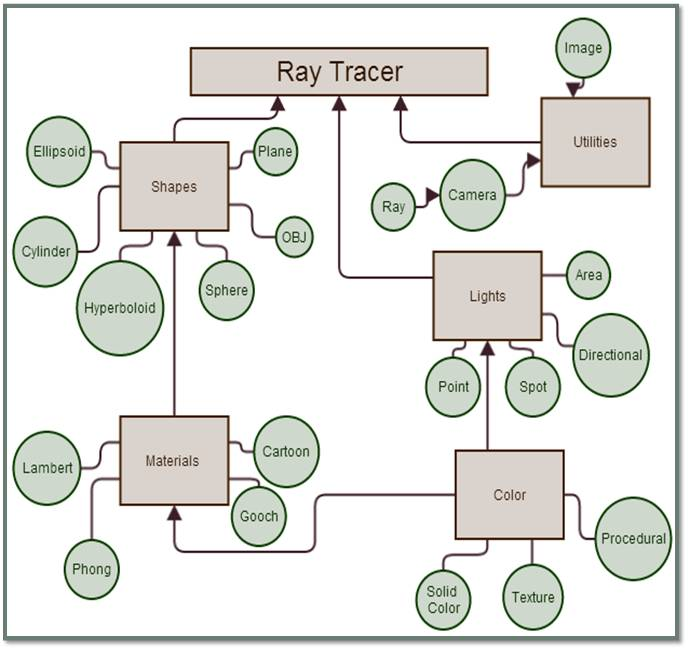
\includegraphics[height=3.0in]{figures/rayTracerStructure.jpg}
\caption{Diagram of the Parenting/Dependency Structure of the Ray Casting Program}
\label{fig:RayTracerDependencies}
\end{figure}

The method used by the researcher are simple and straightforward.  For each coding language, notes were kept that outlined the difficulties and roadblocks met specifically caused by each language.  To provide continuity between each coding process, the same coding theories and fundamentals were be kept.  It can be argued that an object oriented approach to software development is one of the best practices because it is a well organized and helpful for large coding projects, so this is the approach taken.  This means that classes with specific variables and structures were defined, so that instances of objects could be made.  Wherever possible, the image synthesis process was sub-categorized in order to better organize the information needed for the process, which can lead to quicker development and troubleshooting after the code has been written. A Diagram of the structure for the ray tracing program can be seen in Figure \ref{fig:RayTracerDependencies}.

\begin{figure}[ht]
\centering
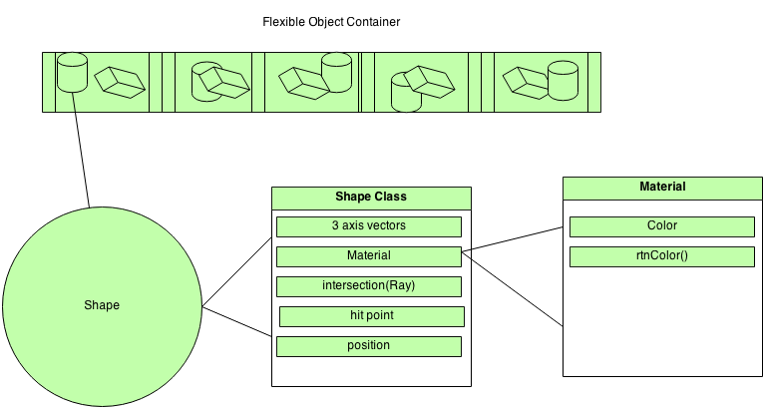
\includegraphics[height=3.0in]{figures/data_structure.png}
\caption{Diagram of the strived for each program Structure of a Ray Casting Program}
\label{fig:RayTracerDataStructure}
\end{figure}

Figure \ref{fig:RayTracerDependencies} demonstrates the parenting and dependency relationships between objects in the program.  Since each program was modelled after this conceptualization, measurements of success and difficulty were more clearly defined.  When building large projects it's important visualize the goals and relationships of the project to better understand the process and work smarter while implementing the task.  For each language a similar data structure was also strived for, shown in Figure \ref{fig:RayTracerDataStructure}.  A dynamic data structure that grows and shrinks with the amount of objects added to it along with a agnostic data structure type was desired for this project.  As we will see in the next section, this was intuitively most similar to the functionality of a ray casters.  In addition to having a program architecture and data structure, the milestones established by the researcher that segments image synthesis theory within four categories also provided a structured approach to analyzing and reporting the conclusions used for each language.  More details on the milestones can be found in the following section.

By determining the difficulty in implementing Figure \ref{fig:RayTracerDependencies} and Figure \ref{fig:RayTracerDataStructure} along with using that class structure to further implement the image synthesis milestones of Preliminary Preparations, Direct Illumination, Ray Tracing/Distributed Ray Tracing, and Indirect Illumination, a detailed report has been collected that informs the results collected and reported in this thesis.  